%


\documentclass{beamer}
% alternatives: scrartcl, article or report


\usetheme{default}
\usecolortheme{default}
\usefonttheme[onlymath]{serif}



%%%%% PACKAGES

% small tweaks and nicer typography
\usepackage{microtype}
\usepackage{hyperref}

% changes language to German
% gives proper date, and correct hyphenation
%\usepackage[ngerman]{babel}
%\uselanguage{German}
%\languagepath{German}

% basic math stuff
\usepackage{mathtools}
\usepackage{amssymb}
\usepackage{amsthm}
%\usepackage{tikz-cd}
\usepackage{cancel}
\usepackage{cases}
\usepackage{dsfont}
\usepackage{delimset} % for nice delimiters
\usepackage{centernot}


% tikz
\usepackage{tikz}
\usepackage{pgfplots}
\usetikzlibrary{positioning}
%\usetikzlibrary{patterns}
%\usetikzlibrary{babel}
\tikzset{>=stealth}
\usepackage{wrapfig}

% Plotting
\usepackage{pgfplots}

% code
%\usepackage{listings}
%\usepackage{pythonhighlight}
%\usepackage{algorithm}
%\usepackage{algpseudocode}
\usepackage{algorithm2e}
\RestyleAlgo{algoruled}

\usepackage[backend=bibtex, style=ieee]{biblatex}
%\usepackage{biblatex}
%\addbibresource{mybib.bib}

% dealing with figures
%\usepackage[figurename=Abb.]{caption}
\usepackage{subcaption}
\usepackage{wrapfig}

% display quotes correctly
\usepackage{csquotes}

% allow for any font-size, alternative mathpazo
\usepackage{mathptmx}

% color
\usepackage{xcolor}

%%%% Graphics %%%%%

%\graphicspath{{Plots/}}

%\newcommand{\tikzmark}[3][]{\tikz[remember picture,baseline] \node [anchor=base,#1](#2) {$#3$};}

%\usepackage{booktabs}
%\usepackage{bm}
%\usepackage{minted}

% for inkscape images
%\usepackage{pdftricks}
%\begin{psinputs}
%   \usepackage{pstricks}
%   \usepackage{multido}
%\end{psinputs}
%\usepackage[pdf]{pstricks}
%\usepackage{import}



% images
\usepackage{graphicx}
\graphicspath{ {./Plots} }

% tikz
\usepackage{tikz}
\usetikzlibrary{positioning}
\usetikzlibrary{babel}
\tikzset{>=stealth}
\newcommand{\tikzmark}[3][]{\tikz[remember picture,baseline] \node [anchor=base,#1](#2) {$#3$};}


% Tikz librarys
\usetikzlibrary{datavisualization}
\usetikzlibrary{datavisualization.formats.functions}
%\usetikzlibrary{external}
%\tikzexternalize[prefix=../Resources/]



%%%%% CONFIGURATION

% prevents automatic line breaks inside of equations
% since it looks bad
\binoppenalty = \maxdimen
\relpenalty   = \maxdimen


%%%%%% PGFPLOTS %%%%%%%%%%%

%\usepgfplotslibrary{grouplots}
\usepgfplotslibrary{dateplot}


%%%%% CUSTOM COMMANDS

% real numbers via \R
% complex numbers via \C
% general field via \K
\def\C{\mathbb{C}}
\def\R{\mathbb{R}}
\def\K{\mathbb{K}}
\def\F{\mathbb{F}}
\def\Q{\mathbb{Q}}
\def\Z{\mathbb{Z}}
\def\N{\mathbb{N}}
\def\H{\mathbb{H}}
\def\e{\varepsilon}

\newcommand{\cA}{\mathcal{A}}
\newcommand{\cB}{\mathcal{B}}
\newcommand{\cC}{\mathcal{C}}
\newcommand{\cD}{\mathcal{D}}
\newcommand{\cE}{\mathcal{E}}
\newcommand{\cF}{\mathcal{F}}
\newcommand{\cG}{\mathcal{G}}
\newcommand{\cH}{\mathcal{H}}
\newcommand{\cI}{\mathcal{I}}
\newcommand{\cJ}{\mathcal{J}}
\newcommand{\cK}{\mathcal{K}}
\newcommand{\cL}{\mathcal{L}}
\newcommand{\cM}{\mathcal{M}}
\newcommand{\cN}{\mathcal{N}}
\newcommand{\cO}{\mathcal{O}}
\newcommand{\cP}{\mathcal{P}}
\newcommand{\cQ}{\mathcal{Q}}
\newcommand{\cR}{\mathcal{R}}
\newcommand{\cS}{\mathcal{S}}
\newcommand{\cT}{\mathcal{T}}
\newcommand{\cU}{\mathcal{U}}
\newcommand{\cV}{\mathcal{V}}
\newcommand{\cW}{\mathcal{W}}
\newcommand{\cX}{\mathcal{X}}
\newcommand{\cY}{\mathcal{Y}}
\newcommand{\cZ}{\mathcal{Z}}

\newcommand{\bA}{\mathbb{A}}
\newcommand{\bB}{\mathbb{B}}
\newcommand{\bC}{\mathbb{C}}
\newcommand{\bD}{\mathbb{D}}
\newcommand{\bE}{\mathbb{E}}
\newcommand{\bF}{\mathbb{F}}
\newcommand{\bG}{\mathbb{G}}
\newcommand{\bH}{\mathbb{H}}
\newcommand{\bI}{\mathbb{I}}
\newcommand{\bJ}{\mathbb{J}}
\newcommand{\bK}{\mathbb{K}}
\newcommand{\bL}{\mathbb{L}}
\newcommand{\bM}{\mathbb{M}}
\newcommand{\bN}{\mathbb{N}}
\newcommand{\bO}{\mathbb{O}}
\newcommand{\bP}{\mathbb{P}}
\newcommand{\bQ}{\mathbb{Q}}
\newcommand{\bR}{\mathbb{R}}
\newcommand{\bS}{\mathbb{S}}
\newcommand{\bT}{\mathbb{T}}
\newcommand{\bU}{\mathbb{U}}
\newcommand{\bV}{\mathbb{V}}
\newcommand{\bW}{\mathbb{W}}
\newcommand{\bX}{\mathbb{X}}
\newcommand{\bY}{\mathbb{Y}}
\newcommand{\bZ}{\mathbb{Z}}



\newcommand{\hu}{\hat{u}}
\newcommand{\hv}{\hat{v}}
\newcommand{\hV}{\hat{V}}
\newcommand{\hw}{\hat{w}}
\newcommand{\hW}{\hat{W}}
\newcommand{\hA}{\hat{A}}
\newcommand{\hC}{\hat{C}}
\newcommand{\hR}{\hat{R}}
\newcommand{\hQ}{\hat{Q}}
\newcommand{\hq}{\hat{q}}
\newcommand{\hp}{\hat{p}}
\newcommand{\hl}{\hat{\ell}}
\newcommand{\hlambda}{\hat{\lambda}}
\newcommand{\ha}{\hat{a}}
\newcommand{\hb}{\hat{b}}
\newcommand{\hs}{\hat{s}}


\newcommand{\tiS}{\tilde{S}}
\newcommand{\tiu}{\tilde{u}}
\newcommand{\tih}{\tilde{h}}
\newcommand{\tix}{\tilde{x}}
\newcommand{\tiy}{\tilde{y}}
\newcommand{\tis}{\tilde{s}}
\newcommand{\tie}{\tilde{\e}}
\newcommand{\tisigma}{\tilde{\sigma}}


\newcommand{\bartheta}{\bar{\theta}}
\newcommand{\barU}{\bar{U}}



%%%%%%%%%%    Math operators    %%%%%%%%%%%%%%%%%%%%%%%%%%%


\newcommand{\dif}[1]{\,\mathrm{d} #1}
%\newcommand{\norm}[1]{\lVert #1 \rVert}
%\newcommand{\abs}[1]{\left| #1 \right|}
\newcommand{\bnorm}[1]{\left\lVert #1\right\rVert}
\newcommand{\vii}[2]{\ensuremath{\begin{bmatrix}#1 \\ #2 \end{bmatrix}}}
\newcommand{\mii}[4]{\ensuremath{\begin{bmatrix}#1&#2 \\ #3&#4 \end{bmatrix}}}
\newcommand{\mc}[1]{\mathcal{#1}}

\newcommand{\one}{\mathds{1}}
\newcommand{\bigO}{\mathcal{O}}


\DeclareMathOperator{\Image}{Image}
\DeclareMathOperator{\Vspan}{Span}
\DeclareMathOperator{\Erf}{erf}
\DeclareMathOperator{\Id}{Id}             % identity morphism
% \DeclareMathOperator{\ker}{ker}           % kernel
\DeclareMathOperator{\rg}{rg}             % image
\DeclareMathOperator{\defekt}{def}             % defect
\DeclareMathOperator{\im}{im}             % image
\DeclareMathOperator{\Hom}{Hom}           % homomorphisms
\DeclareMathOperator{\End}{End}           % endomorphisms
\DeclareMathOperator{\Span}{Span}         % linear span
\DeclareMathOperator{\grad}{\nabla}         % gradient
\DeclareMathOperator{\diam}{diam}         % gradient
\DeclareMathOperator{\Tr}{Tr}       	  % trace
\DeclareMathOperator{\diver}{Div}			% divergence
\DeclareMathOperator{\supp}{supp}			% support
\DeclareMathOperator{\dist}{dist}			% distance
\DeclareMathOperator{\inter}{int}			% interiour
\DeclareMathOperator{\epi}{epi}			% epigraph
\DeclareMathOperator{\hyp}{hyp}			% hypograph
\DeclareMathOperator{\Lip}{Lip}			% lipschitz konstant
\DeclareMathOperator{\graph}{graph}			% graph
\DeclareMathOperator{\sgn}{sgn}			% sign
\DeclareMathOperator{\BMO}{BMO}			% BMO
\DeclareMathOperator{\mean}{mean}			% BMO
%\DeclareMathOperator{\B}{B}			% BMO


% \vect{ x // y // z } for a column vector with entries x, y, z
% similarly for larger vectors
% in this code:  1 = number of arguments
%               #1 = first argument
\newcommand{\vect}[1]{\begin{bmatrix} #1 \end{bmatrix}}

% \conj{z} for complex conjugation
\newcommand{\conj}{\overline}

%counter of current constant number:    
\newcounter{constant} 
%defines a new constant, but does not typeset anything:
\newcommand{\newconstant}[1]{\refstepcounter{constant}\label{#1}} 
%typesets named constant:
\newcommand{\useconstant}[1]{c_{\ref{#1}}}

%%%%%%% GENERAL STYLE %%%%%%%%%%%%%%%%%%

\setcounter{tocdepth}{3}
\setcounter{secnumdepth}{0}


%%%%%%% COLORS %%%%%%%%%%%%%%%%%%%%%%%%


\newcommand{\black}{\color{black}}


%%%%%% TITLE PAGE
%
%\subject{Specialised Course in Integration Theory, VT23}
%\title{Assignment Chapter 3.5}
%\author{Theo Koppenhöfer}
%\date{\today}
%
%
%%%%%% The content starts here %%%%%%%%%%%%%
%
%
%\begin{document}
%
%\maketitle
%
%
%%\nocite{*}
%\printbibliography
%
%\end{document}


%%%%%%% GENERAL STYLE %%%%%%%%%%%%%%%%%%
%
%\setcounter{tocdepth}{3}
%\setcounter{secnumdepth}{0}


% modify beamer template
\setbeamercolor{footline}{fg=blue}
\setbeamerfont{footline}{size={\fontsize{10}{12}}}
\setbeamertemplate{navigation symbols}{}

%\setbeamertemplate{navigation symbols}{%
%    \usebeamerfont{footline}%
%    \usebeamercolor[fg]{footline}%
%    \hspace{1em}%
%    \raisebox{4pt}[0pt][0pt]{\insertframenumber/\inserttotalframenumber}
%}

%\setbeamertemplate{footline}{
%	\vspace*{0.1cm}
%	\hspace*{0.01cm}
%	\insertsection
%	\hfill\insertframenumber/\inserttotalframenumber
%	\hspace*{0.1cm}
%}

\setbeamertemplate{footline}[page number]

% modify handling of bibliography
\setbeamertemplate{bibliography entry title}{}
\setbeamertemplate{bibliography entry location}{}
\setbeamertemplate{bibliography entry note}{}

\setbeamertemplate{bibliography item}[text]


%%%%% allow for proofs over multiple slides

\makeatletter
\newenvironment<>{proofs}[1][\proofname]{%
    \par
    \def\insertproofname{#1\@addpunct{.}}%
    \usebeamertemplate{proof begin}#2}
  {\usebeamertemplate{proof end}}
\makeatother


%%%%%%% theorem environments

\newtheorem{proposition}{Proposition}

%%%%%% TITLE PAGE
%
%\subject{Specialised Course in Integration Theory, VT23}
%\title{Assignment Chapter 3.5}
%\author{Theo Koppenhöfer}
%\date{\today}
%
%
%%%%%% The content starts here %%%%%%%%%%%%%
%
%
%\begin{document}
%
%\maketitle
%
%
%%\nocite{*}
%\printbibliography
%
%\end{document}


%%%%% TITLE PAGE

\subject{, VT23}
\title{%Junzi Zhang, Brendan O'Donoghue, Stephen Boyd: 
Globally Convergent Type-I Anderson Acceleration for Non-Smooth Fixed-Point Iterations}
%\subtitle{}
\author{Theo Koppenhöfer}
\date{Lund \\[1ex] \today}


%\SetAlFnt{\small}
\addbibresource{bibliography.bib}



\begin{document}

\frame[plain]



% Frame 2
\frame[plain]{\titlepage}

% Frame 3
\frame[plain]{ \frametitle{Table of contents} \tableofcontents }

\section{An introductory example}
\begin{frame}

\end{frame}

\section{AA-II}
\subsection{AA-II}
\begin{frame}
%	\IncMargin{1em}
	\begin{algorithm}[H]
	\caption{General AA}\label{alg:cap}
	\SetKwInOut{Input}{Input}
	
	\Input{$x^0\in\R^n$, $f\colon\R^n\to\R^n$}
	\BlankLine
	\For{$k=0,1,\dots$}{
	  Choose $m_k\in\{0,\dots,k\}$\;
	  Choose $\alpha^k\in \R^{m_k}$ such that $\sum_i\alpha_i^k=1$\;
	  $f_k =f\brk*{x_k}$
	  $x_{k+1} = \sum_i \alpha_i^kf_{k-m_k+i}$\;
	}
	\end{algorithm}
\end{frame}


\begin{frame}
%	\IncMargin{1em}
	\begin{algorithm}[H]
	\caption{General AA}
	\SetKwInOut{Input}{Input}
	\color{gray}
	\Input{$x^0\in\R^n$, $f\colon\R^n\to\R^n$}
	\BlankLine
	\For{$k=0,1,\dots$}{
	  Choose $m_k\in\{0,\dots,k\}$\;
	  Choose $\alpha^k\in \R^{m_k}$ such that $\sum_i\alpha_i^k=1$ {\color{black} and such that $\alpha$ minimises $\norm{\sum_i\alpha^k_ig^i}_2$}\;
	  $f_k =f\brk*{x_k}$\;
	  $x_{k+1} = \sum_i \alpha_i^kf_{k-m_k+i}$\;
	}
	\end{algorithm}
\end{frame}

\begin{frame}
	\frametitle{AA-II}
	Define residual $g=\Id-f\colon\R^n\to\R^n$ and $g_k = g(x_k)$.
	Choose $\alpha\in\R^{m_k}$ such that it minimises
	\begin{align*}
		\norm{\sum_i\alpha^k_ig_i}_2
	\end{align*}
	and
	\begin{align*}
		\sum_i\alpha^k_i = 1\,.
	\end{align*}
	It can be shown that then
	\begin{align*}
		x_{k+1} = \sum_i \alpha_i^kf\brk*{x_{k-m_k+i}} = x_k-H_kg_k
	\end{align*}
	for some $H_k\in\R^{n\times m_k}$ such that $H_k$ minimises $\norm{H_k-\Id}_F$.
\end{frame}


\subsection{AA-I}
\begin{frame}
	\frametitle{AA-I}
\end{frame}

\begin{frame}
%	\IncMargin{1em}
	\begin{algorithm}[H]
	\caption{AA-I}
	\SetKwInOut{Input}{Input}
	\color{gray}
	\Input{$x^0\in\R^n$ and $f\colon\R^n\to\R^n$}
	\BlankLine
	Set $H_0=\Id$, $x_1=f\brk{x_0}$.
	
	\For{$k=0,1,\dots$}{
		Set $g_k= g(x_{k})$,
		$s_{k-1}= x_k-x_{k-1}$ and
		$y_{k-1}= g_k-g_{k-1}$.
		
		Set $\hs_{k-1}= s_{k-1}-\sum_{i=0}^{k-2}\frac{\hs_i^\top s_{k-1}}{\norm{\hs_i}^2}s_i$.
		
		Set $H_k = H_{k-1}+\frac{(s_{k-1}-H_{k-1}y_{k-1})s_{k-1}^\top H_{k-1}}{\hs_{k-1}^\top H_{k-1}y_{k-1}}$ and $x_{k+1}= x_k-H_kg_k$.
		
	}
	\end{algorithm}
\end{frame}

\section{Modifications to AA-I}
\subsection{Powell-type regularisation}

\begin{frame}	
	\frametitle{Powell-type regularisation}
	Note that $B_k$ may be singular. To solve this set
	\begin{align*}
		\tiy_k=\theta_ky_k+(1-\theta_k)B_ks_k
	\end{align*}
	where
	\begin{align*}
		\theta_k = \phi_{\bartheta}(\eta_k)
	\end{align*}
	and
	\begin{align*}
		\phi_{\bartheta}(\eta) = \begin{cases}
			\frac{1-\sgn(\eta)\bartheta}{1-\eta} &\text{ if }\abs{\eta}<\bartheta \\
			1 &\text{ else }
		\end{cases} \qquad
		\eta_k = \frac{\hs_k^\top H_ky_k}{\norm{\hs_k}^2}
	\end{align*}
\end{frame}

\begin{frame}
	One can obtain
	\begin{lemma}[Powell-type regularisation]
		Let $s_k\in\R^n$, $B_0=\Id$, and inductively
		\begin{align*}
			B_{k+1} = B_k+\frac{\brk{\tiy_k-B_ks_k}\hs_k^\top}{\hs_k^\top s_k}
		\end{align*}
		with $\hs_k$ and $\tiy_k$ defined as before. If this is well-defined then $\abs{\det\brk{B_k}}\geq \theta^k>0$ and $B_k$ is invertible.
	\end{lemma}
	\begin{proof}
		See \cite[Lemma 2]{ZhaAA}.
	\end{proof}
\end{frame}

\begin{frame}
%	\IncMargin{1em}
	\begin{algorithm}[H]
	\caption{AA-I with Powell-like-regularisation}
	\SetKwInOut{Input}{Input}
	\color{gray}
	\Input{$x^0\in\R^n$, $f\colon\R^n\to\R^n$ and ${\black\bartheta\in(0,1)}$}
	\BlankLine
	Set $H_0=\Id$, $x_1=f\brk{x_0}$.
	
	\For{$k=0,1,\dots$}{
		Set $g_k= g(x_{k})$,
		$s_{k-1}= x_k-x_{k-1}$ and
		$y_{k-1}= g_k-g_{k-1}$.
		
		Set $\hs_{k-1}= s_{k-1}-\sum_{i=0}^{k-2}\frac{\hs_i^\top s_{k-1}}{\norm{\hs_i}^2}s_i$.
		
		{\black
		Set $\eta_{k-1}= \frac{\hs_{k-1}^\top H_{k-1}y_{k-1}}{\norm{\hs_{k-1}}^2}$, 
		$\theta_{k-1}=\phi_{\bartheta}(\eta_{k-1})$
		and $\tiy_{k-1}=\theta_{k-1}y_{k-1}-(1-\theta_{k-1})g_{k-1}$.
		}
		
		Set $H_k = H_{k-1}+\frac{(s_{k-1}-H_{k-1}\tiy_{k-1})}{\hs_{k-1}^\top H_{k-1}\tiy_{k-1}}$ and $x_{k+1}= x_k-H_kg_k$.
		
	}
	\end{algorithm}
\end{frame}

\subsection{Restarting iteration}
\begin{frame}
	\frametitle{Restarting iteration}
	Note that
	\begin{align*}
		B_{k+1} = B_k+\frac{\brk{\tiy_k-B_ks_k}\hs_k^\top}{\hs_k^\top s_k}
	\end{align*}
	is ill-defined iff $\norm{\hs_k}^2=\hs_k^\top s_k=0$, i.e.\ $\hs_k=0$. This can occur for $m_k>n$ as we then have $\hs_k=0$ by linear dependence.
	If we reset $m_k=0$ if $m_k=m+1$ or $\norm{\hs_{k-1}}<\tau\norm{s_{k-1}}$ for some $\tau\in(0,1)$
	then 
	$$g_k\neq 0 \implies s_k=-B_kg_k\neq 0\implies \hs_k\neq 0\,.$$
\end{frame}

\begin{frame}
	\begin{lemma}[Restarting iteration]
		If we additionally choose $m_k$ by the rule above we have
		\begin{align*}
			\norm{B_k}\leq 3\brk*{\frac{1+\bartheta+\tau}{\tau}}^m-2\,.
		\end{align*}
	\end{lemma}
	\begin{proof}
		See \cite[Lemma 3]{ZhaAA}.
	\end{proof}
\end{frame}

\begin{frame}
%	\IncMargin{1em}
	\begin{algorithm}[H]
	\caption{AA-I with Powell-like-regularisation and Restarting}
	\SetKwInOut{Input}{Input}
	\color{gray}
	\Input{$x^0\in\R^n$, $f\colon\R^n\to\R^n$, {\color{black}$m \in\N$ }and $\bartheta{, \black\tau}\in(0,1)$}
	\BlankLine
	Set $H_0=\Id$, $x_1=f\brk{x_0}$, $m_0 = 0$.
	
	\For{$k=0,1,\dots$}{
		Set $g_k= g(x_{k})$,
		$m_k= m_{k-1}+1$, 
		$s_{k-1}= x_k-x_{k-1}$ and
		$y_{k-1}= g_k-g_{k-1}$.
		
		Set $\hs_{k-1}= s_{k-1}-\sum_{i=k-m_k}^{k-2}\frac{\hs_i^\top s_{k-1}}{\norm{\hs_i}^2}s_i$.
		
		{\black
		\If{$m_k=m+1$ or $\norm{\hs_{k-1}}<\tau\norm{s_{k-1}}$}{
			Set $m_k=0$, $\hs_{k-1}= s_{k-1}$ and $H_{k-1}=\Id$.
		}
		}
		Set $\eta_{k-1}= \frac{\hs_{k-1}^\top H_{k-1}y_{k-1}}{\norm{\hs_{k-1}}^2}$, 
		$\theta_{k-1}=\phi_{\bartheta}(\eta_{k-1})$
		and $\tiy_{k-1}=\theta_{k-1}y_{k-1}-(1-\theta_{k-1})g_{k-1}$.
		
		Set $H_k = H_{k-1}+\frac{(s_{k-1}-H_{k-1}\tiy_{k-1})}{\hs_{k-1}^\top H_{k-1}\tiy_{k-1}}$ and $x_{k+1}= x_k-H_kg_k$.
		
	}
	\end{algorithm}
\end{frame}


\subsection{Safeguarding steps}
\begin{frame}
	\frametitle{Safeguarding steps}
	To guarantee the decrease in $\norm{g_k}$ one can interleave the AA-I steps with Krasnoselskii-Mann steps which are given by
	\begin{align*}
		x_{k+1}= (1-\alpha)x_k +\alpha f(x_k)
	\end{align*}
	for some fixed $\alpha\in(0,1)$.
\end{frame}

\SetAlFnt{\footnotesize}

\begin{frame}
%	\IncMargin{1em}
	\begin{algorithm}[H]
	\caption{AA-I with Powell-like-regularisation, Restarting and Safeguarding}\label{alg:aa1-prs}
	\SetKwInOut{Input}{Input}
	\color{gray}
	\Input{$x^0\in\R^n$, $f\colon\R^n\to\R^n$,$m \in\N$, $\bartheta, \tau, {\color{black}\alpha}\in(0,1)$, {\color{black}safe-guarding constants $D,\e>0$}}
	\BlankLine
	Set $H_0=\Id$, $x_1={\black\tix_1=f\brk{x_0}}$, $m_0 = {\color{black}n_{AA}=0}$ and ${\color{black}\barU=\norm{g_0}_2}$.
	
	\For{$k=0,1,\dots$}{
		Set $g_k= g(x_{k})$,
		$m_k= m_{k-1}+1$, 
		$s_{k-1}= {\black\tix_k}-x_{k-1}$ and
		$y_{k-1}= g({\black\tix_k})-g_{k-1}$.
		
		Set $\hs_{k-1}= s_{k-1}-\sum_{i=k-m_k}^{k-2}\frac{\hs_i^\top s_{k-1}}{\norm{\hs_i}^2}s_i$.
		
		\If{$m_k=m+1$ or $\norm{\hs_{k-1}}<\tau\norm{s_{k-1}}$}{
			Set $m_k=0$, $\hs_{k-1}= s_{k-1}$ and $H_{k-1}=\Id$.
		}
		Set $\eta_{k-1}= \frac{\hs_{k-1}^\top H_{k-1}y_{k-1}}{\norm{\hs_{k-1}}^2}$, 
		$\theta_{k-1}=\phi_{\bartheta}(\eta_{k-1})$
		and $\tiy_{k-1}=\theta_{k-1}y_{k-1}-(1-\theta_{k-1})g_{k-1}$.
		
		Set $H_k = H_{k-1}+\frac{(s_{k-1}-H_{k-1}\tiy_{k-1})}{\hs_{k-1}^\top H_{k-1}\tiy_{k-1}}$ and $\tix_{k+1}= x_k-H_kg_k$.
		
		{\color{black}
		\uIf{$\norm{g_k}\leq D\barU(n_{AA}+1)^{-(1+\e)}$}{
			Set $x_{k+1}=\tix_{k+1}$ and $n_{AA}= n_{AA}+1$.
		}
		\Else{
			Set $x_{k+1}= (1-\alpha)x_k +\alpha f(x_k)$
		}
		}
	}
	\end{algorithm}
\end{frame}

\section{Convergence result}

\begin{frame}
	\frametitle{Convergence result}
	\begin{theorem}[Convergence]
		Let $x_k$ be generated by algorithm \ref{alg:aa1-prs} then $x_k\xrightarrow{k\to\infty}x_*$ and $f(x_*)=x_*$ is a fixed point.
	\end{theorem}
\end{frame}


\section{Numerical experiments}

\subsection{Regularised logistic regression}

\begin{frame}
	\frametitle{Regularised logistic regression}
	We take $x\in\R^{2000\times 500}=, y\in\R^{2000}$ with  from the UCI Madelon dataset. The aim is to minimise
	\begin{align*}
		F(\theta) = \frac{1}{2000}\sum_{i}\log\brk{1+\sum_jy_ix_{ij}\theta_j}+\frac{\lambda}{2}\norm{\theta}^2
	\end{align*}
	with gradient descent, i.e.\
	\begin{align*}
		f(\theta) = \theta-\alpha\nabla F(\theta)
	\end{align*}
	for some $\alpha\in(0,2/L)$.
\end{frame}

\begin{frame}
	\begin{figure}
		\centering
		% This file was created with tikzplotlib v0.10.1.
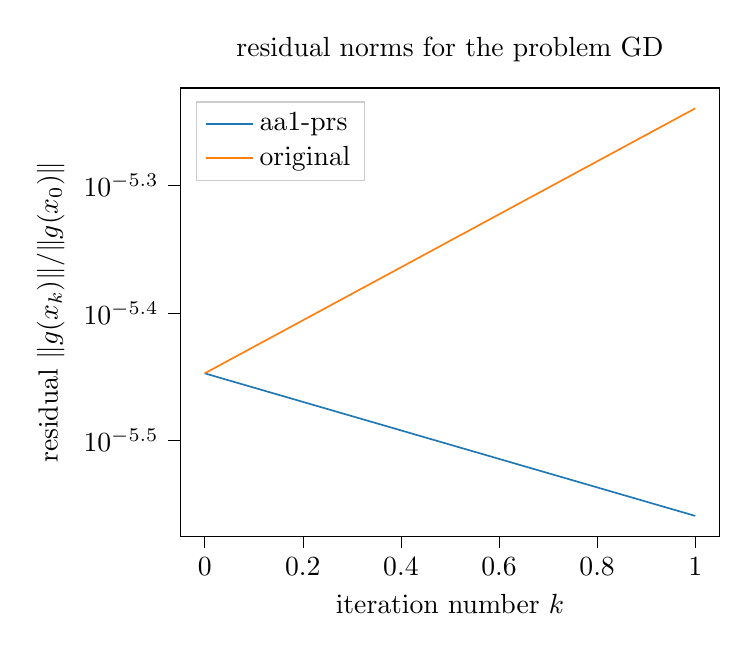
\begin{tikzpicture}

\definecolor{darkgray176}{RGB}{176,176,176}
\definecolor{darkorange25512714}{RGB}{255,127,14}
\definecolor{lightgray204}{RGB}{204,204,204}
\definecolor{steelblue31119180}{RGB}{31,119,180}

\begin{axis}[
legend cell align={left},
legend style={
  fill opacity=0.8,
  draw opacity=1,
  text opacity=1,
  at={(0.03,0.97)},
  anchor=north west,
  draw=lightgray204
},
log basis y={10},
tick align=outside,
tick pos=left,
title={residual norms for the problem GD},
x grid style={darkgray176},
xlabel={iteration number \(\displaystyle k\)},
xmin=-0.05, xmax=1.05,
xtick style={color=black},
y grid style={darkgray176},
ylabel={residual \(\displaystyle \norm{g(x_k)}/\norm{g(x_0)}\)},
ymin=2.65702041966114e-06, ymax=5.97564015934737e-06,
ymode=log,
ytick style={color=black}
]
\addplot [semithick, steelblue31119180]
table {%
0 3.56748104631869e-06
1 2.75673117031559e-06
};
\addlegendentry{aa1-prs}
\addplot [semithick, darkorange25512714]
table {%
0 3.56748104631869e-06
1 5.75950172251125e-06
};
\addlegendentry{original}
\end{axis}

\end{tikzpicture}

		\caption{Residual norms for the logistic regression problem.}
	\end{figure}
\end{frame}

\subsection*{Facility location}

\begin{frame}
	
\end{frame}

\begin{frame}
	\begin{figure}
		\centering
		% This file was created with tikzplotlib v0.10.1.
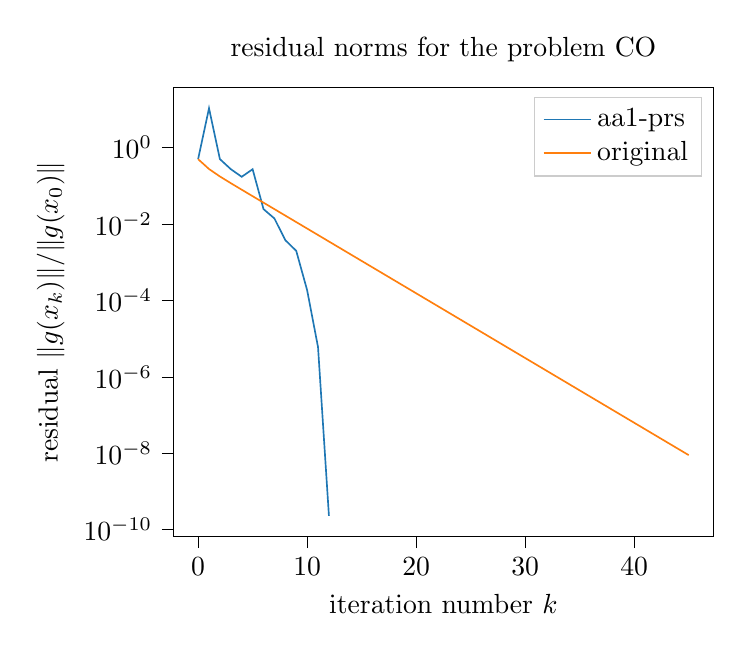
\begin{tikzpicture}

\definecolor{darkgray176}{RGB}{176,176,176}
\definecolor{darkorange25512714}{RGB}{255,127,14}
\definecolor{lightgray204}{RGB}{204,204,204}
\definecolor{steelblue31119180}{RGB}{31,119,180}

\begin{axis}[
legend cell align={left},
legend style={fill opacity=0.8, draw opacity=1, text opacity=1, draw=lightgray204},
log basis y={10},
tick align=outside,
tick pos=left,
title={residual norms for the problem CO},
x grid style={darkgray176},
xlabel={iteration number \(\displaystyle k\)},
xmin=-2.25, xmax=47.25,
xtick style={color=black},
y grid style={darkgray176},
ylabel={residual \(\displaystyle \norm{g(x_k)}/\norm{g(x_0)}\)},
ymin=6.75895940356585e-11, ymax=36.2782620232941,
ymode=log,
ytick style={color=black}
]
\addplot [semithick, steelblue31119180]
table {%
0 0.495588643966115
1 10.6285804099101
2 0.495588643966115
3 0.270976993907102
4 0.171122093577714
5 0.269797398098345
6 0.0244274510783268
7 0.0138820384409515
8 0.00375628732223015
9 0.00197677871866153
10 0.000185167940418084
11 5.98577437452288e-06
12 2.30701834855331e-10
};
\addlegendentry{aa1-prs}
\addplot [semithick, darkorange25512714]
table {%
0 0.495588643966115
1 0.273098074040799
2 0.174466335318158
3 0.11649433193869
4 0.0786362295023986
5 0.0532118801882059
6 0.03602627220658
7 0.0243931681808116
8 0.0165164582075084
9 0.0111830322229492
10 0.00757175864069581
11 0.00512660584009843
12 0.00347104542446171
13 0.00235011304996452
14 0.00159116754254216
15 0.00107731371027646
16 0.000729403537312378
17 0.000493847817458106
18 0.00033436294236866
19 0.000226382552482769
20 0.000153273699758866
21 0.000103774880955939
22 7.02613984375745e-05
23 4.75708921225878e-05
24 3.22081497092301e-05
25 2.1806714540865e-05
26 1.47643621283447e-05
27 9.99629653346881e-06
28 6.76805013547979e-06
29 4.58234728535713e-06
30 3.10250456411087e-06
31 2.10056854640408e-06
32 1.42220200407257e-06
33 9.62910033449992e-07
34 6.5194376579213e-07
35 4.4140227007474e-07
36 2.988539421256e-07
37 2.02340772792762e-07
38 1.36995985545873e-07
39 9.27539189678542e-08
40 6.2799576221216e-08
41 4.2518815038927e-08
42 2.87876035730159e-08
43 1.94908134041768e-08
44 1.31963658200782e-08
45 8.93467750652024e-09
};
\addlegendentry{original}
\end{axis}

\end{tikzpicture}

		\caption{Residual norms for the facility location problem.}
	\end{figure}
\end{frame}

\section{Sources}

\begin{frame}[allowframebreaks]
	\frametitle{Sources}
	\nocite{*}
%	\bibliographystyle{plain}
%	\bibliography{bibliography}
	\printbibliography
\end{frame}


\begin{frame}[plain]
	\begin{center}
		\Large{{Thank you for your attention.}}
	\end{center}
\end{frame}

\frame[plain]

\end{document}
